W tym rozdziale zostanie opisana konfiguracja pierwotna robota z wyszczególnieniem elementów, które mogą być problemem przy dalszym rozwoju możliwości tego urządzenia.
\begin{figure}[!ht]
 \centering
 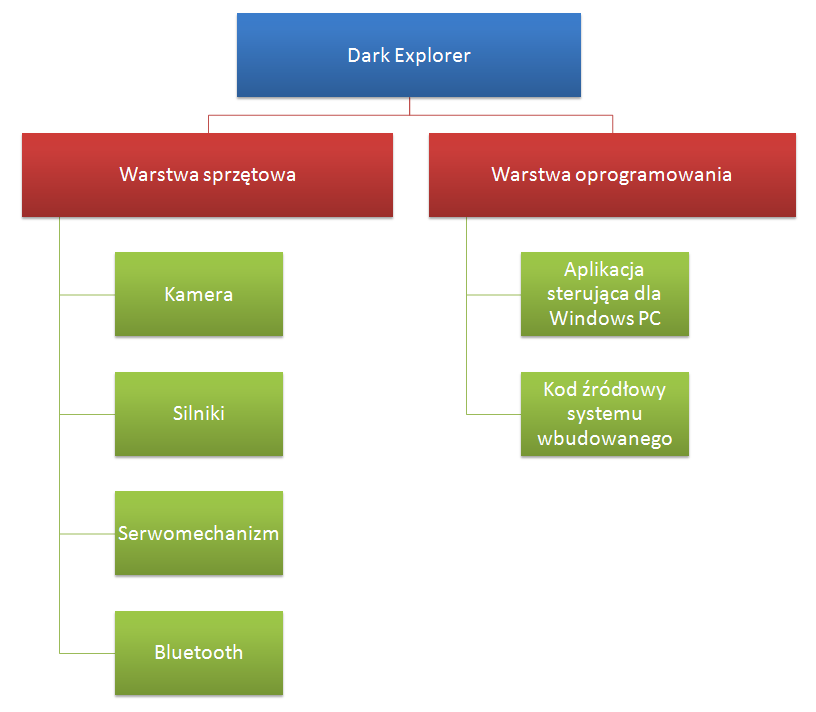
\includegraphics[height=125mm]{../images/ch02/kmak_platform.png}
 \caption{Struktura platformy robota mobilnego zrealizowanej w ramach
 poprzedniej pracy magisterskiej\cite{KmakMScThesis2009}}
 \label{fig:KmakPlatform}
\end{figure}

\section{Analiza sprzętu}
Dark Explorer jest autonomicznym robotem mobilnym z wbudowaną kolorową kamerą cyfrową VGA. Jego podstawowe możliwości to:
\begin{itemize}
 \item jazda ze zmienną prędkością w przód, tył, lewo oraz prawo
 \item komunikacja z urządzeniami zewnętrznymi przy pomocy technologii bluetooth
 \item wykonywanie zdjęć z maksymalną rozdzielczością $160x100$ pikseli w kolorze oraz $320x200$ pikseli w odcieniach szarości
 \item poruszanie wieżyczką na której zainstalowana jest kamera
 \item wykrywanie prostych wzorców przy pomocy analizy obrazu oraz podążanie za nimi
\end{itemize}

\subsection{Elementy elektroniczne}
Dark Explorer został wyposażony w mikrokontroler zarządzający AT91Sam7s256 o częstotliwości pracy zegara maksymalnie do 50 MHz oraz wbudowanej szybkiej pamięci SRAM 64 kB. Mikrokontroler ten jest bogaty w różnego rodzaju urządzenia peryferyjne takie jak na przykład: TWI\footnote{TWI -- Two Wire Interfece znany również jako $I^{2}C$, interfejs szeregowej komunikacji danych}, RTT\footnote{RTT -- Real Time Timer, służy do odmierzania dłuższych odcinków czasu}, PDC\footnote{PDC -- Peripheral DMA Controller, kontroler DMA}, AIC\footnote{AIC -- Advanced Interrupt Controller, kontroler przerywań}, PWM\footnote{PWM -- Pulse Width Modulation Controller}, ADC\footnote{ADC -- Analog to Digital Converter, konwerter analogowo cyfrowy}. To tylko część z nich. Dzięki tak wielkiemu wyborowi urządzeń peryferyjnych mikrokontroler ten daje nam duże możliwości rozwoju konfiguracji. Częstotliwość pracy mikrokontrolera ARM7 jest wystarczająca do zadań przez niego wykonywanych.

Większość elementów elektronicznych robota jest umieszczonych na płycie głównej zaprojektowanej przez autora projektu robota. Jest ona bardzo dobrze przemyślana ponieważ pozwala na wykorzystywanie urządzeń peryferyjnych mikrokontolera w praktycznie dowolny sposób. Większość wyjść oraz wejść mikrokontrolera nie jest połączona na stałe z konkretnymi podzespołami Dark Explorera lecz poprzez zworki, które pozwalają podłączanie i odłączanie poszczególnych urządzeń.

\begin{figure}[!ht]
 \centering
 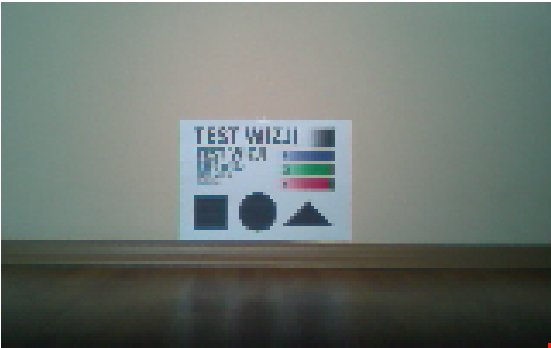
\includegraphics[height=50mm]{../images/ch02/160x100C.jpg}
 \caption{Obraz wykonany przy pomocy kamery zamontowanej w robocie. 160 x 100 pikseli w kolorze. \cite{KmakMScThesis2009}}
 \label{fig:160x100C}
\end{figure}

Twórca Dark Explorera wyposażył go kamerę cyfrową o maksymalnej rozdzielczości $640x480$ pikseli. Jest to urządzenie $PO6040$ firmy Pixelplus. Można go konfigurować przy pomocy interfejsu $I^{2}C$. W konfiguracji pierwotnej robot potrafi odbierać zdjęcia o maksymalnej rozdzielczości $320x200$ pikseli w odcieniach szarości(rys. \ref{fig:320x200BW}) oraz $160x100$ pikseli w kolorze (rys. \ref{fig:160x100C}). Tak niskie rozdzielczości nie są wystarczające do wykrywania i tym bardziej rozpoznawania twarzy na obrazie dlatego też konieczna jest poprawa tych parametrów.

W skład robota wchodzą także silniki napędowe, serwomechanizm, dioda mocy oraz moduł bluetooth. Wszystkie te elementy muszą być podłączone do mikrokontrolera przez konkretne wejścia/wyjścia. Z tego powodu do dyspozycji osób przeprowadzających dalszy rozwój robota pozostało jedynie pięć wejść/wyjść cyfrowych oraz trzy wejścia analogowe. Jest to kolejna przeszkoda którą trzeba będzie pokonać.

\begin{figure}[!ht]
 \centering
 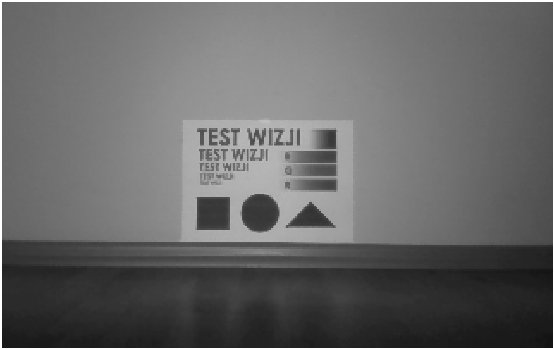
\includegraphics[height=50mm]{../images/ch02/320x200B&W.jpg}
 \caption{Obraz wykonany przy pomocy kamery zamontowanej w robocie. 320 x 200 pikseli w odcieniach szarości \cite{KmakMScThesis2009}}
 \label{fig:320x200BW}
\end{figure}

Robot mobilny komunikuje się z urządzeniami zewnętrznymi przy pomocy modułu bluetooth BTM-222 firmy Rayson. Maksymalna przepustowość danych z jaką potrafi działać wynosi 3Mb/s. Obsługiwane przez niego interfejsy to: USB, UART oraz PCM. Mikrokontroler komunikuje się z modułem bluetooth przy pomocy interfejsu UART o maksymalnej przepustowości 460,8 kb/s. Jak widać takie rozwiązanie nie wykorzystuje pełnych możliwości modułu BTM-222. Bardziej efektywne byłoby skorzystanie z interfejsu USB który potrafi przesyłać dane z prędkością maksymalną od 1,5Mb/s w standardzie USB 1.0 do 5Gb/s w standardzie USB 3.0. Aby dokonać zmiany interfejsu komunikacyjnego pomiędzy mikrokontrolerem a modułem bluetooth konieczna jest ingerencja w konstrukcję płyty głównej robota, gdyż BTM-222 jest przylutowany bezpośrednio do niej \ref{fig:BTM222}.

\begin{figure}[!ht]
 \centering
 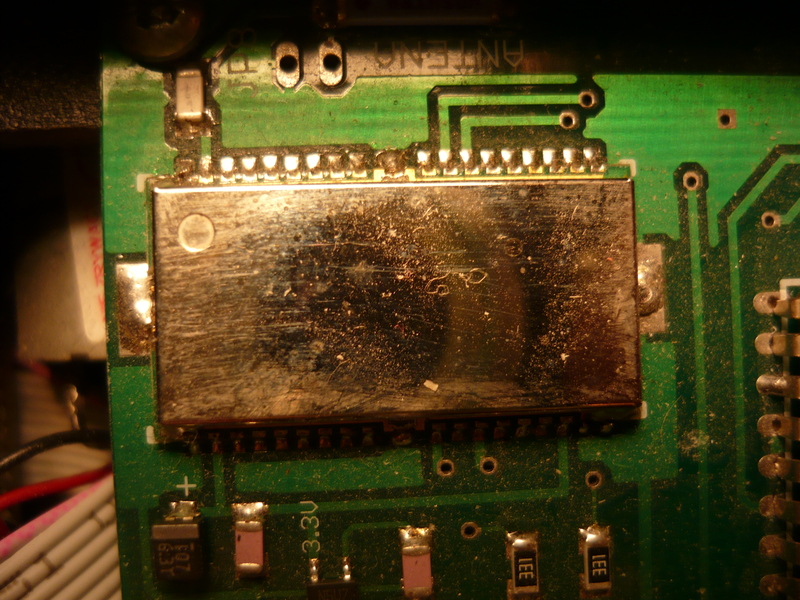
\includegraphics[height=50mm]{../images/ch02/btm-222.jpg}
 \caption{Zdjęcie modułu bluetooth zamontowanego na płycie głównej robota.}
 \label{fig:BTM222}
\end{figure}

\subsection{Elementy mechaniczne}
Konstrukcja obudowy Dark Explorera została wykonana z tworzywa sztucznego i jest dopasowana do elementów które zostały zaprojektowane przez autora. Wewnątrz obudowy nie ma miejsca na jakiekolwiek nowe podzespoły, dlatego też konieczna będzie jej modyfikacja (rys. \ref{fig:KmakMainBoard}).

\begin{figure}[!ht]
 \centering
 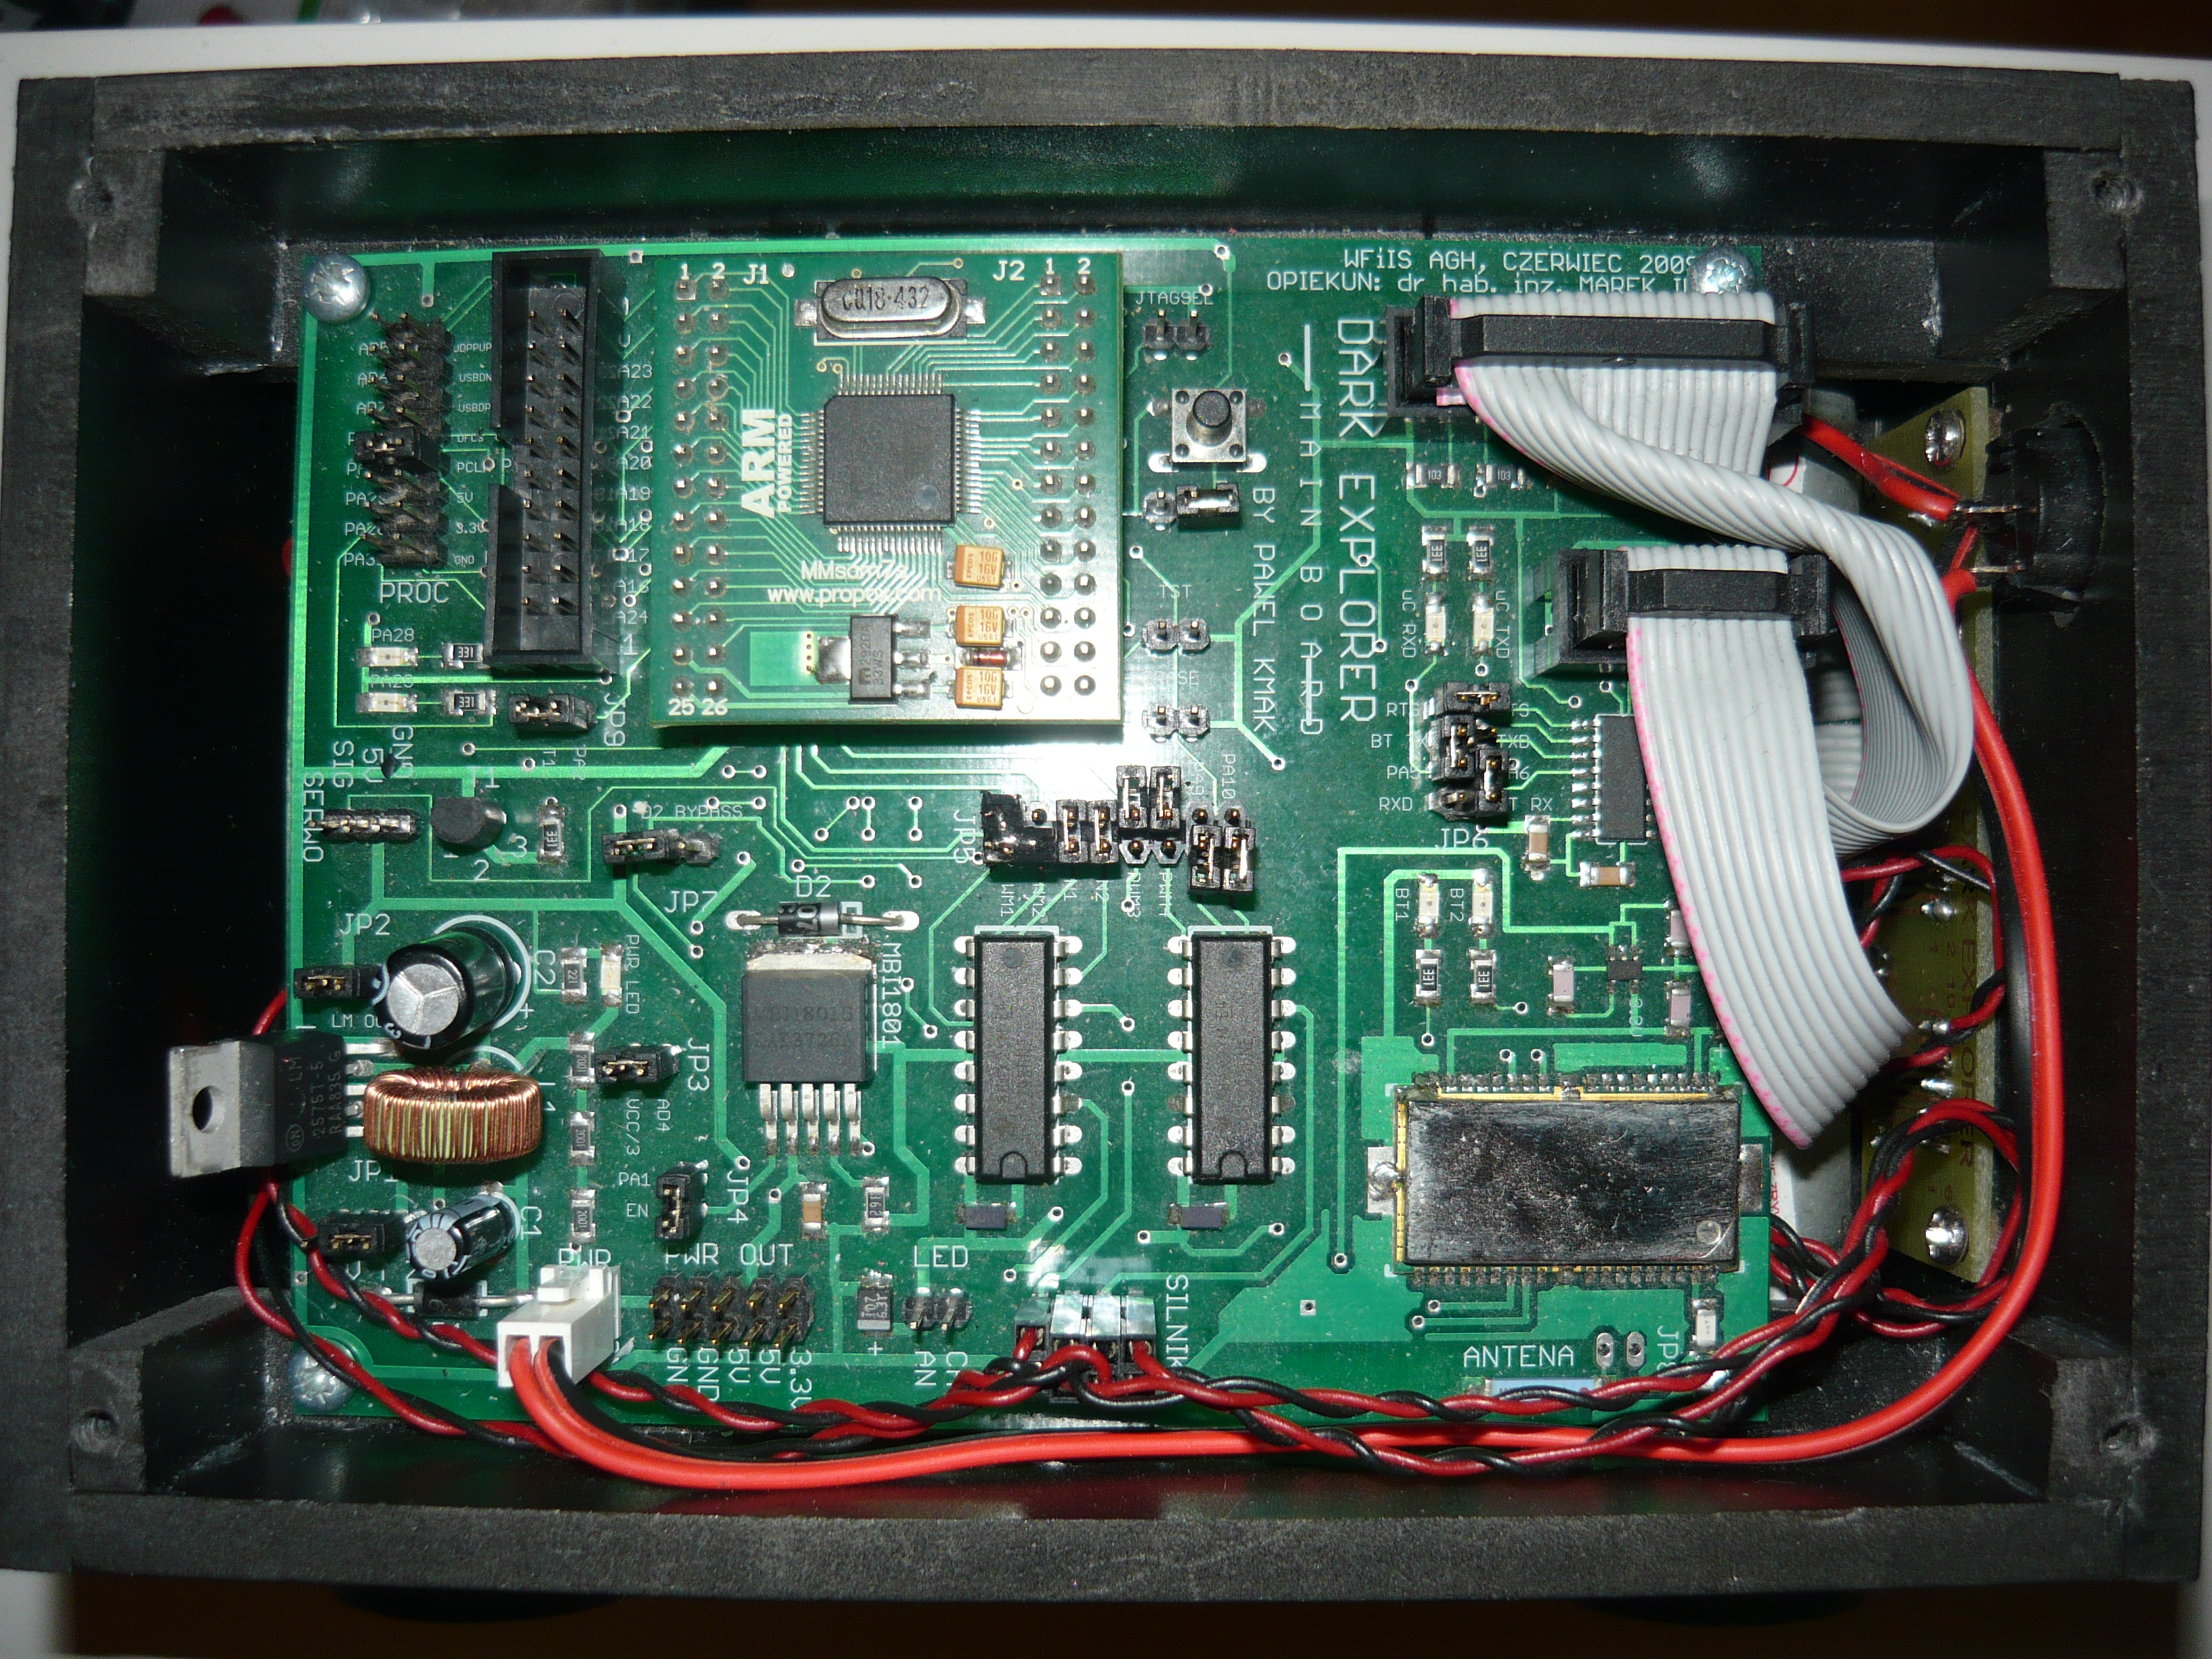
\includegraphics[height=75mm]{../images/ch02/main_board.jpg}
 \caption{Widok na płytę główną Dark Explorer'a}
 \label{fig:KmakMainBoard}
\end{figure}

Podczas testów konfiguracji pierwotnej zauważono lekkie kłopoty robota z poruszaniem się po gładkich powierzchniach. Najprawdopodobniej jest to spowodowane kółkami (rys. \ref{fig:KmakWheel}) zamontowanymi przy robocie, które tracą przyczepność na nieco bardziej śliskim podłożu. Możliwe, że podczas rozwoju robota, konieczna będzie ich wymiana w celu zapewnienia dobrej przyczepności i poprawnego toru jazdy urządzenia.

\begin{figure}[!ht]
 \centering
 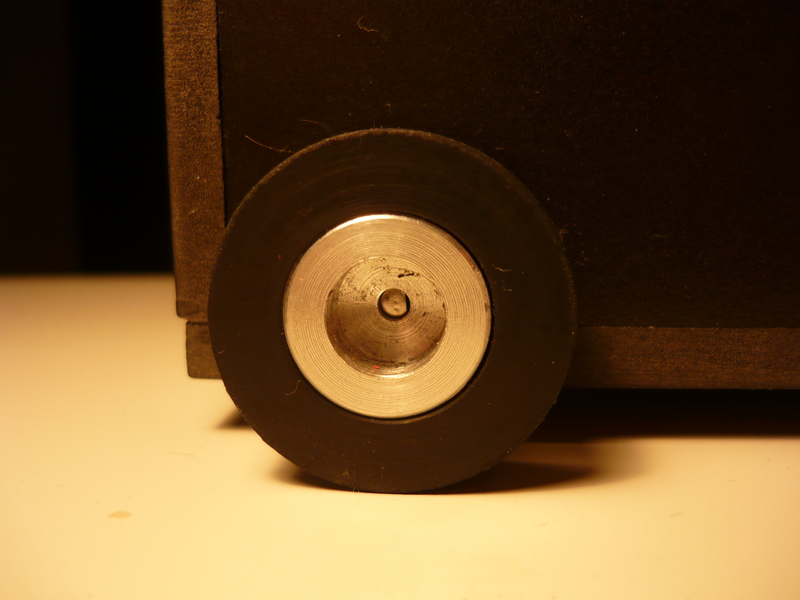
\includegraphics[height=75mm]{../images/ch02/wheel.jpg}
 \caption{Koło napędowe Dark Explorer'a}
 \label{fig:KmakWheel}
\end{figure}
